% kapitel2.tex
\definecolor{light-gray}{gray}{0.93}
\chapter{Analyse von RAD-Seq-Daten} \label{chapter:kap2}
\section{Problemstellung} \label{sec:probl}

Ausgangsmaterial für RAD-Seq-Analysen sind die Reads aus in der Regel gepoolten Probengemischen mehrerer Individuen. Durch entsprechende Barcodemarkierungen können die Reads den einzelnen Individuen zugeordnet werden. Die Verwendung gepoolter Probengemische macht das Verfahren kostengünstiger und zeitsparender als die meisten anderen NGS-Verfahren. Die Reads stammen aus dem gesamten Genom, wobei sie nur kleinere Sequenzabschnitte zwischen den Schnittstellen der Restriktionsenzyme repräsentieren und damit nicht das gesamte Genom abbilden. Ein deutlicher Vorteil des Verfahrens besteht darin, die Reads ohne Kenntnis eines Referenzgenoms möglichen Loci zuordnen zu können. Auch die Loci und ihre Sequenz sind somit anfangs unbekannt und werden erst durch die Analyse ermittelt.\\

Das RAD-Sequencing-Verfahren bedingt, dass durch die Restriktionsenzyme die DNA nur  innerhalb spezifischer Sequenzen geschnitten wird und dass durch PCR und Sequenzierung mehrere Reads erzeugt werden, die jeweils vom gleichen Locus stammen. Das hier implementierte Tool NodeRAD \cite{noderad} stellt einen Prototypen dar, der im Gegensatz zu derzeit etablierten RADSeq-Tools, wie beispielsweise dem Tool Stacks \cite{catchen_2013}, mit Hilfe von nur zwei Parametern diese Zuordnung realisiert. Das Clustering der Reads sowie die Identifizierung und Locizuordnung sollen dabei unter Berücksichtigung der Ploidie ohne weiteres Vorwissen allein auf Grundlage der Sequenzierfehlerrate und Heterozygotiewahrscheinlichkeit erfolgen. Die ermittelten Loci sollen für anschließende Diversitätsanalysen zur Verfügung stehen. 

\section{Formale Definition der Problemstellung} \label{sec:formal}

Gegeben sei eine Menge von Reads eines Individuums $ D = (s_{1}, \dots , s_{m}) \in \{A,\,C,\,G,\,T,\}^{k^m}$ mit der Readlänge $k$. In den Reads sind zudem für jede Base Informationen zur Qualität der Sequenzierung $ Q = (q_{1}, \dots , q_{m}) \in {[0,\,1]}^{k^m}$ enthalten. Weiterhin seien für Substitutionen, Insertionen und Deletionen die Heterozygotiewahrscheinlichkeiten $\eta=(\eta_{sub},\, \eta_{ins},\, \eta_{del}) $ und für Indels die Sequenzierfehlerraten $\epsilon=(\epsilon_{ins},\, \epsilon_{del})$ gegeben. Ebenso ist die Ploidie $\phi$ des untersuchten Organismus bekannt. In der vorliegenden Arbeit wird im Model und beim implementierten Prototypen ein diploider Chromosomensatz vorausgesetzt, für höherploide Organismen ist eine Anpassung hinsichtlich des Sequenzalignments notwendig (siehe Kap. \ref{sec:ausblick}). \\

Ziel ist die Zuordnung der Reads zu den Loci unter Berücksichtigung von $\epsilon$ und $\eta$ sowie die Ausgabe der Menge der ermittelten Loci mit den Sequenzen der beteiligten Allele. Dabei soll die Menge von Loci gefunden werden, welche die beobachteten Reads am besten erklären kann, das heißt welche die höchste Wahrscheinlichkeit in Zusammenschau mit $\epsilon$ und $\eta$ besitzt. \\

\section{Lösungsansatz und Modell} \label{sec:solution}

Das Problem wird als gerichteter Graph betrachtet (siehe Kap. \ref{subsec:sol_graph}), dessen Knoten die einzelnen Reads beinhalten und dessen Kanten auf einem Sequenzalignment der Reads basieren. Für die Zuordnung der Reads soll das Problem in Teilprobleme aufgeteilt werden, für jedes Teilproblem wird dann eine Lösung ermittelt. Der Graph wird daher entsprechend seiner Zusammenhangskomponenten partitioniert. Die in einer Zusammenhangskomponente vorkommenden Sequenzen werden in Abhängigkeit von konfigurierbaren Schwellenwerten als Kandidatenallele betrachtet und jeweils mit sämtlichen Reads der Zusammenhangskomponente verglichen. Dabei sollen diejenigen Allele identifiziert werden, von denen die übrigen Reads der Komponente am wahrscheinlichsten durch Sequenzierfehler entstanden sind (Kap. \ref{subsec:sol_allele_lh}). Die Likelihoodberechnung hierfür wird durch die Basenqualität der Reads und Sequenzierfehlerrate bestimmt und erfolgt über alle Kombinationen möglicher Häufigkeitsverteilungen der Allele (Allele-Fractions). \\

Die Allele-Fraction mit der höchsten Likelihood $\Theta_{max\_lh}$ soll anschließend für die Zuordnung der Loci verwendet werden (Kap. \ref{subsec:sol_loci_lh}). Hierfür wird die Likelihood für alle Loci-Kombinationen bestimmt, welche zu der ermittelten $\Theta_{max\_lh}$ passen. Für die Berechnung der Likelihoods der Locizuordnung werden die Heterozygotiewahrscheinlichkeiten verwendet. Die Loci-Kombination mit der größten Likelihood wird schließlich als Lösung der betreffenden Zusammenhangskomponente ausgegeben.\\

Für jede Zusammenhangskomponente wird auf diese Weise die wahrscheinlichste Lösung ermittelt, deren Komposition von Loci die beobachteten Reads innerhalb der Zusammenhangskomponente am besten erklären kann. Die Loci mit maximaler Likelihood aus allen Zusammenhangskomponenten werden schließlich durch NodeRAD im VCF-Format ausgegeben. Eine Übersicht der einzelnen Schritte des Workflows findet sich in \autoref{fig:workflow_all}. Die dort dargestellten Schritte werden im Folgenden näher erläutert. \\

%https://texample.net/tikz/examples/labs-schema/
\usetikzlibrary{shadows,arrows}
% Layer des Diagramms
\pgfdeclarelayer{background}
\pgfdeclarelayer{foreground}
\pgfsetlayers{background,main,foreground}

% Eigenschaften der Blöcke 
\tikzstyle{blocktxt}=[draw, text width=6.0em, text centered,
minimum height=1.5em,drop shadow]
\tikzstyle{blockitem} = [blocktxt, fill=green!40, text width=8em, minimum width=10em,
minimum height=3em, rounded corners, drop shadow]
\tikzstyle{ioitem} = [blocktxt, fill=white, text width=8em, minimum width=10em,
minimum height=3em, rounded corners, drop shadow]
\tikzstyle{sectiontxt} = [above, text = black, text width=6em, text centered]
\tikzstyle{dashedline} = [draw, thick, color=black, -latex', dashed]
\tikzstyle{line} = [draw, thick, color=red, -latex']
\tikzstyle{ur}=[draw, text centered, minimum height=0.01em]

% Distanzen
\newcommand{\blockdist}{1.3}
\newcommand{\edgedist}{1.5}

\newcommand{\blockitem}[2]{node (p#1) [blockitem]
	{\textbf{\textit{#2}}}}

\newcommand{\ioitem}[2]{node (p#1) [ioitem]
	{\textbf{\textit{#2}}}}

% Eigenschaften der DNA-Abbildung
\newcommand{\bond}[3]{
	\draw[very thick, #1] (#3, 0) -- (#3, 0.35);
	\draw[very thick, densely dotted] (#3, 0.35) -- (#3, 0.65);
	\draw[very thick, #2] (#3, 0.65) -- (#3, 1);
}
% Hintergrundfeld
\newcommand{\background}[5]{%
	\begin{pgfonlayer}{background}
		% Hintergrundfeld obere linke Ecke
		\path (#1.west |- #2.north)+(-3.3,0.3) node (a1) {};
		% Hintergrundfeld untere rechte Ecke
		\path (#3.east |- #4.south)+(+0.5,-0.25) node (a2) {};
		% Hintergrundeigenschaften
		\path[fill=blue!20,rounded corners, draw=black]
		(a1) rectangle (a2);
		\path (a1.east |- a1.south) +(-3.0,-1.0) node (u1)[sectiontxt]
		{\textbf{\textit{#5}}};
\end{pgfonlayer}}

\newcommand{\out}[3]{%
	\path [dashedline] (#1.east) -- node [above]
	{\scriptsize Output: #2} (#3);}

\begin{figure}[]
	\begin{center}
		\begin{tikzpicture}[scale=0.64,transform shape]
			% https://github.com/PetarV-/TikZ/tree/master/DNA
			\path \ioitem {1}{Reads\\
				\begin{tikzpicture}[scale=0.6,transform shape]
				\bond{red}{blue}{0.1}
				\bond{red}{blue}{0.25}
				\bond{red}{blue}{0.4}
				\bond{blue}{red}{1.1}
				\bond{blue}{red}{1.25}
				\bond{blue}{red}{1.4}
				\bond{red}{blue}{2.1}
				\bond{red}{blue}{2.25}
				\bond{red}{blue}{2.4}
				\bond{blue}{red}{3.1}	
				\bond{blue}{red}{3.25}
				\bond{blue}{red}{3.4}
				\bond{red}{blue}{4.1}
				\bond{red}{blue}{4.25}
				\bond{red}{blue}{4.4}
				\braid[rotate=90,style strands={1}{red, very thick},style strands={2}{blue, very thick}] (tst) at (0, 0) s_1 s_1 s_1 s_1 ;
				\end{tikzpicture}
			};
			\path (p1.south)+(-2.5,-2.0) \blockitem{2}{\hyperref[step1txt]{\color{green!40}..}1. Adapter trimming};\phantomsection\label{step1}
			\path (p2.south)+(2.5,-1.2) \blockitem{3}{\hyperref[step2txt]{\color{green!40}..}2.\phantomsection\label{step2} Quality \\control};
			\path (p3.south)+(-2.5,-1.2) \blockitem{5}{\hyperref[step3txt]{\color{green!40}..}3.\phantomsection\label{step3} Sequence alignment};
			\path (p3.west)+(4.75,-3.8) \blockitem{4}{\hyperref[step4txt]{ 4}.\phantomsection\label{step4} Build graph};
			\path (p3.east)+(+9.8, 0.0) node (ur1)[ur] {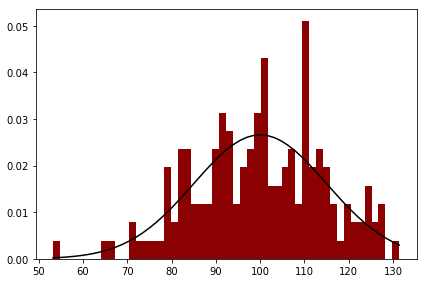
\includegraphics[width=2.0cm]{bilder/qc_reports_icon_5.png}};
			\path (p4.south)+(0.0,-1.5) \blockitem{6}{\hyperref[step5txt]{\color{green!40}..}5.\phantomsection\label{step5} Connected components};
			\path (p4.east)+(+7.0,0) node (ur2)[ur] {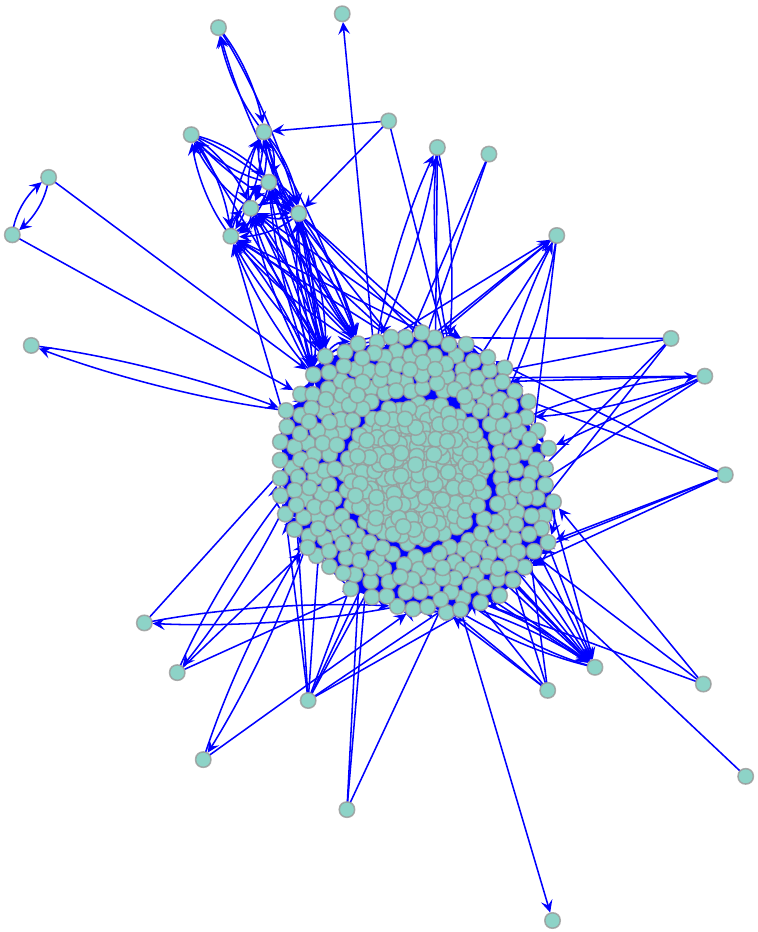
\includegraphics[width=2.0cm]{bilder/big_components_3.png}};
			\path (p6.south)+(-5.5,-1.4) \blockitem{7}{\hyperref[step7txt]{\color{green!40} ..}7.\phantomsection\label{step7} Allele \\combinations};
			\path (p6.south)+(0.0,-1.4) \blockitem{8}{\hyperref[step6txt]{\color{green!40}..}6.\phantomsection\label{step6} Candidate \\alleles};
			\path (p6.east)+(+6.5,0) node (ur3)[ur] {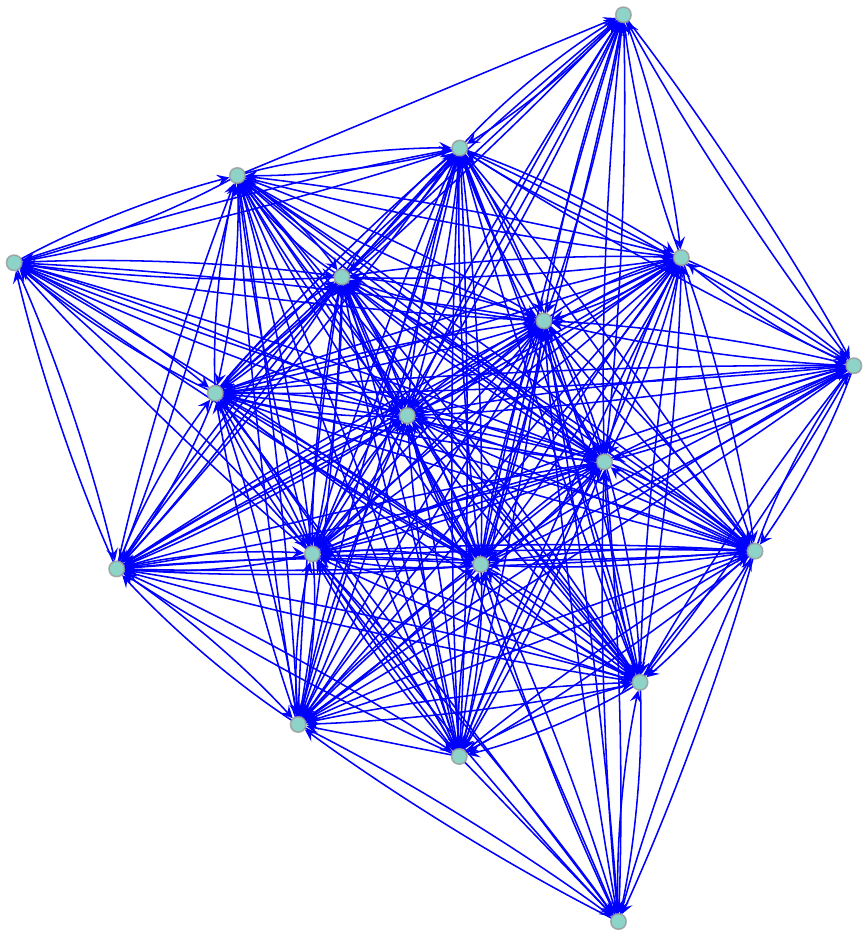
\includegraphics[width=1.0cm]{bilder/small_components_2.png}};				
			\path (p7.south)+(0.0,-3.9) \blockitem{9}{\hyperref[step8txt]{\color{green!40}..}8.\phantomsection\label{step8} Allele fractions};
			\path (p8.south)+(0.0,-1.5)	\blockitem{10}{\hyperref[step9txt]{\color{green!40}..}9.\phantomsection\label{step9} Likelihood of alleles given one read};
			\path (p9.south)+(0.0,-7.64) \blockitem{11}{\hyperref[step14txt]{\color{green!40}.\color{black}1}4.\phantomsection\label{step14} Indicator constraint};
			\path (p10.south)+(0.0,-1.5) \blockitem{12}{\hyperref[step10txt]{\color{green!40}.\color{black}1}0.\phantomsection\label{step10} Likelihood of allele fractions given one read};
			\path (p11.south)+(0.0,-1.5) \blockitem{13}{\hyperref[step13txt]{\color{green!40}..}13.\phantomsection\label{step13} Loci \\combinations};
			\path (p12.south)+(0.0,-1.5) \blockitem{14}{\hyperref[step11txt]{\color{green!40}.\color{black}1}1.\phantomsection\label{step11} Likelihood of allele fractions given all reads};
			\path (p14.south)+(0.0,-1.5) \blockitem{15}{\hyperref[step12txt]{\color{green!40}.\color{black}1}2.\phantomsection\label{step12} Maximum likelihood allele fractions};
			\path (p15.south)+(0.0,-2.0) \blockitem{16}{\hyperref[step15txt]{\color{green!40}.\color{black}1}5.\phantomsection\label{step15} Likelihood \\of an allele given another allele};
			\path (p16.south)+(0.0,-1.8) \blockitem{17}{\hyperref[step16txt]{\color{green!40}.\color{black}1}6.\phantomsection\label{step16} Likelihood of loci given alleles and fractions}; 
			\path (p17.south)+(0.0,-1.3) \blockitem{18}{\hyperref[step17txt]{\color{green!40}.\color{black}1}7.\phantomsection\label{step17} Maximum likelihood loci};
			\path (p18.south)+(0.0,-1.7) \ioitem{19}{\hyperref[step18txt]{\color{white}..}18.\phantomsection\label{step18} VCF \\ 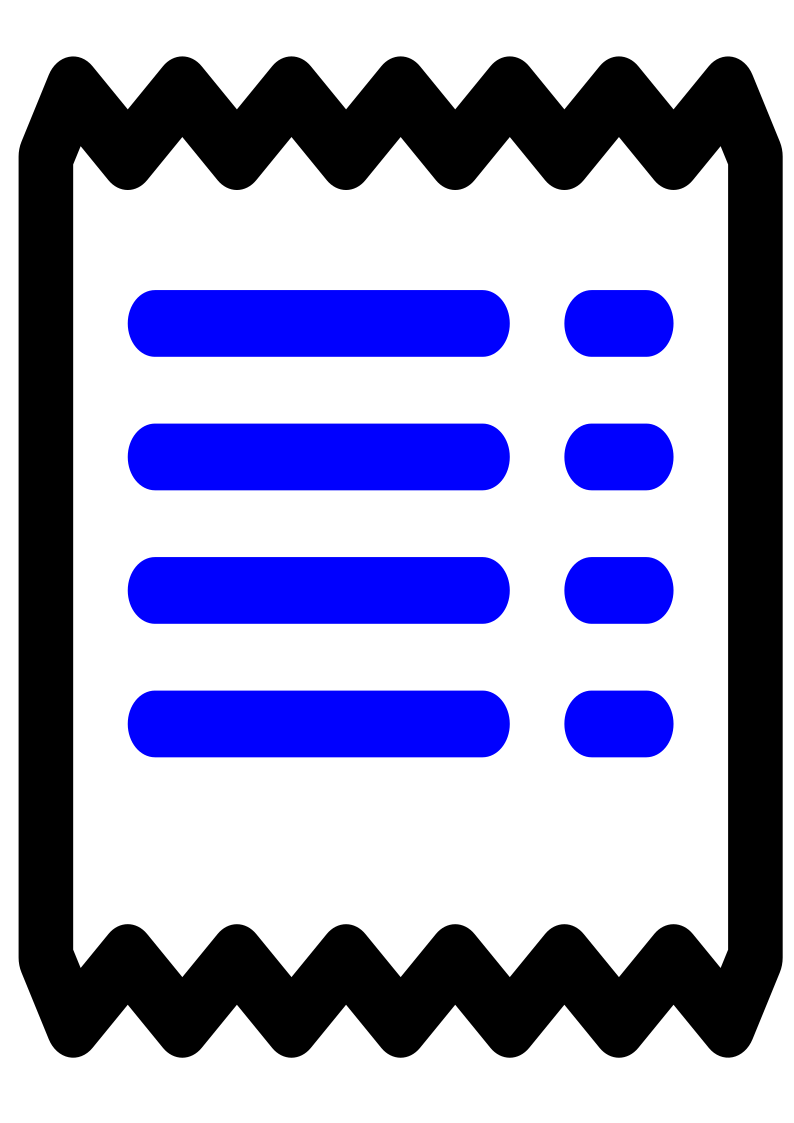
\includegraphics[width=0.9cm]{bilder/list_icon_2.png}\hspace{0.1cm}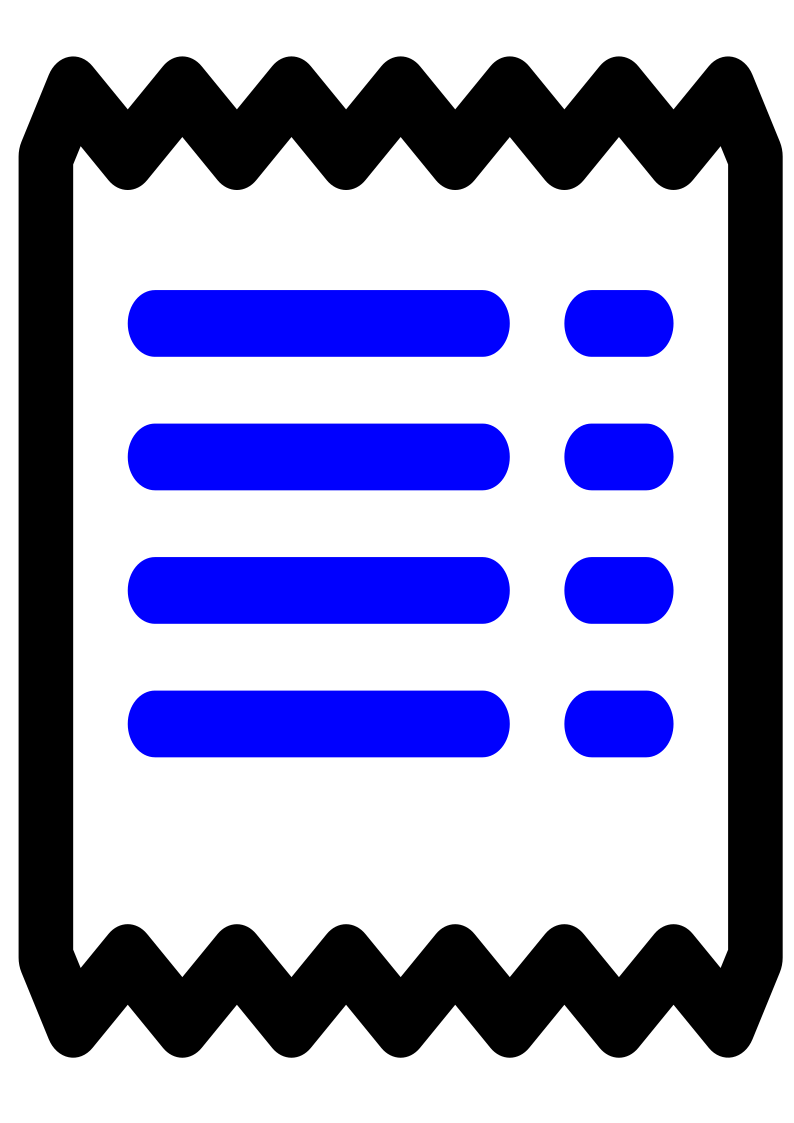
\includegraphics[width=0.9cm]{bilder/list_icon_2.png}\hspace{0.1cm}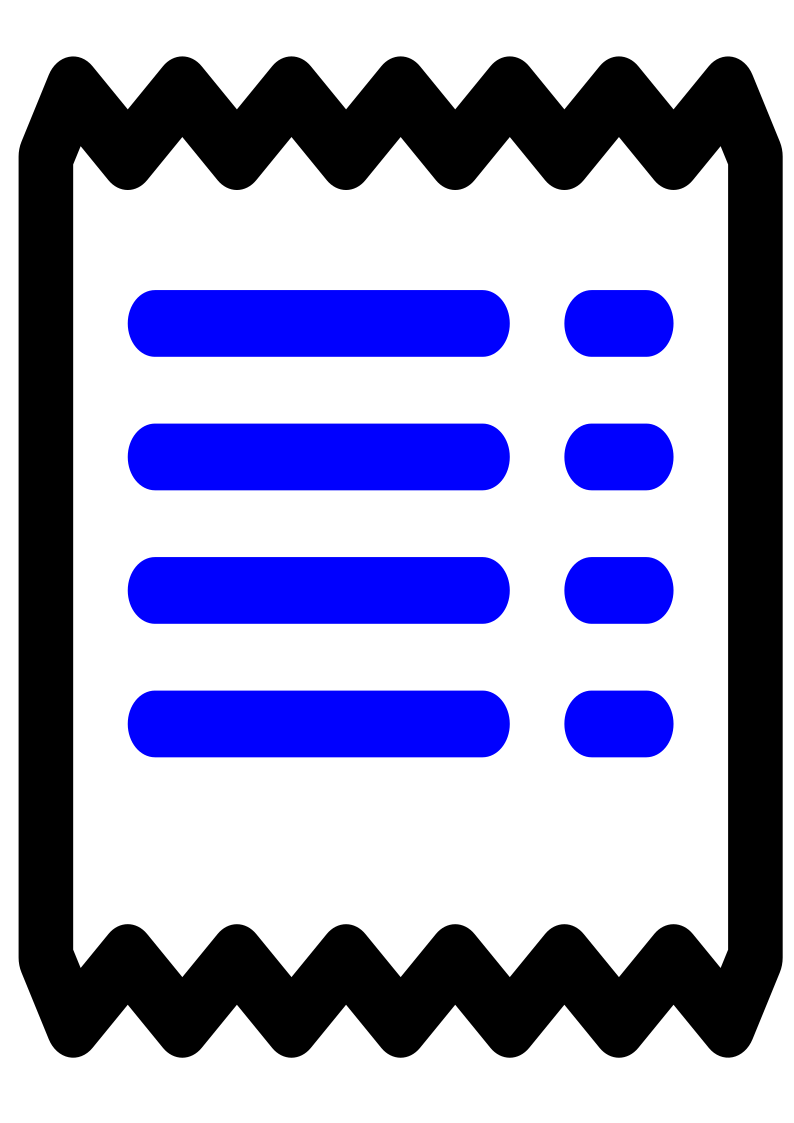
\includegraphics[width=0.9cm]{bilder/list_icon_2.png}};
			
			% Pfeile
			\path [line] (p1.south) -- +(0.0,-0.5) -- +(-2.5,-0.5) -- node [above, midway] {} (p2);
			\path [line] (p1.south) -- +(0.0,-0.5) -- +(+2.83,-0.5) -- node [above, midway] {} (p4);
			\path [line] (p2.south) -- node [above] {} (p3) ;
			\path [line] (p3.south) -- node [above] {} (p5) ;		
			\path [line] (p5.south) -- +(0.0,-1.415) -- node [above, midway] {} (p4.west);		
			\path [line] (p4.south) --node [above] {} (p6);
			\path [line] (p6.south) -- node [above] {} (p8);
			\path [line] (p8.south) -- node [above] {} (p10) ;	
			\path [line] (p10.south) -- node [above] {} (p12) ;	
			\path [line] (p12.south) -- node [above] {} (p14) ;		
			\path [line] (p14.south) -- node [above, midway] {} (p15);
			\path [line] (p15.south) -- node [above] {} (p16) ;     
			\path [line] (p16.south) -- node [above] {} (p17) ;
			\path [line] (p17.south) -- node [above] {} (p18) ;
			\path [line] (p18.south) -- node [above] {} (p19) ;		
			\path [line] (p19.south) -- +(0.0,-0.5) -- +(-8.8,-0.5) -- +(-8.8,27.498) -- node [above] {\color{black}Section 6} (p5.west) ;
			
			\out{p3}{Reports (MultiQC, FastQC)}{ur1}
			\out{p4}{Graph, XML, DOT}{ur2}
			\out{p6}{Subgraphes, XML, DOT}{ur3}
			
			\path [dashedline] (p8.west) -- node [left] {} (p7);
			\path [dashedline] (p7.south) -- node [above] {} (p9) ;
			\path [dashedline] (p9.east) -- node [left] {} (p12.west);
			\path [dashedline] (p9.south) -- node [left] {} (p11.north);
			\path [dashedline] (p11.east) -- node [left] {} (p16.west);
			\path [dashedline] (p13.north) -- node [left] {} (p11.south); 
			
			\background{p3}{p2}{p3}{p5}{Preprocessing}
			\background{p3}{p4}{p4}{p6}{Graph \\construction}
			\background{p3}{p8}{p4}{p15}{Allele Likelihood}
			\background{p3}{p16}{p4}{p18}{Loci Likelihood}
 		\end{tikzpicture}
		\caption{Übersicht der Prozesse des Workflows \cite{tikz_schema, tikz_dna, bootstrap}}
		\label{fig:workflow_all}
	\end{center}
\end{figure}

\subsection{Graph und Zusammenhangskomponenten} \label{subsec:sol_graph}

Im Preprocessing erfolgt die Zuordnung der Reads zu den einzelnen Individuen und die Entfernung der Barcodes aus den Sequenzen (\hyperref[step1]{Schritt 1\phantomsection\label{step1txt}} des Workflows). Anschließend wird in \hyperref[step3]{Schritt 3\phantomsection\label{step3txt}} aus den Reads ein paarweises Sequenzalignment mit Hilfe des Tools Minimap2 ~\cite{li_2018} erzeugt. Hierbei werden alle Reads miteinander verglichen und bei ausreichender Ähnlichkeit ihrer Sequenzen einander zugeordnet. Zusätzlich werden durch Minimap2 die Edit-Distanzen zwischen den jeweils miteinander verglichenen Readsequenzen bestimmt. \\

Wie bereits einleitend erwähnt, wird das Problem als gerichteter Graph $G=(V, \, E)$ mit der Knotenmenge $V$ und der Kantenmenge $E$ betrachtet (\hyperref[step4]{Schritt 4\phantomsection\label{step4txt}} des Workflows). Die Knoten entsprechen dabei den einzelnen Reads. Auf Grundlage des von Minimap2 erzeugtem Sequenzalignment werden die Knoten der Reads durch Kanten verbunden. Die Kanten des Graphen repräsentieren somit den Vergleich der Sequenzen der beiden angrenzenden Reads. Die Anzahl der Kanten kann zusätzlich durch die von Minimap2 bestimmten Edit-Distanzen reguliert werden. Diese soll über einen konfigurierbaren Schwellenwert flexibel wählbar sein und ermöglicht ein zusätzliches Filtern der Kanten zugunsten von  Laufzeit und Effizienz. \\

Da aufgrund des Sequenzalignments nur Reads mit einander verbunden werden, deren Sequenzen eine gewisse Ähnlichkeit zu einander aufweisen und da die RAD-Sequencing-Daten für gewöhnlich mehrere Loci beinhalten, ist der Graph in der Regel nicht zusammenhängend. Dies ermöglicht eine Unterteilung des Gesamtproblems in kleinere Teilprobleme durch Betrachtung der einzelnen Zusammenhangskomponenten des Graphen (\hyperref[step5]{Schritt 5\phantomsection\label{step5txt}}). Für diese Teilprobleme wird dann nach Lösungen gesucht. Da sich die Konstellation der Zusammenhangskomponenten direkt aus dem Sequenzalignment ergibt, sind die so entstandenen Cluster nicht notwendiger Weise nur einem einzigen Locus zuzuordnen. Vielmehr können die einzelnen Zusammenhangskomponenten auch jeweils mehrere Loci beinhalten. \\

\subsection{Approximation von PairHMM mittels Minimap2-Alignments} \label{subsec:phmm_minimap}

Um die wahrscheinlichsten Allele aus der Menge der Reads zu identifizieren und schließlich den wahrscheinlichsten Loci zuordnen zu können, muss ein paarweiser Vergleich der Readsequenzen hinsichtlich ihrer Ähnlichkeit zu einander erfolgen. Bei der Ermittlung der wahrscheinlichsten Allele werden hierfür alle Reads mit den infrage kommenden Allelen verglichen (siehe Kap. \ref{pHMM_alleles}). Bei der Ermittlung der wahrscheinlichsten Loci erfolgt ein paarweiser Vergleich der Allele untereinander (siehe Kap. \ref{pHMM_loci}). Die Kanten des Graphen repräsentieren somit den Vergleich zweier Sequenzen, ihre Gewichtung soll die Ähnlichkeit zwischen den Sequenzen beschreiben. Diese Ähnlichkeit kann durch die Likelihood ausgedrückt werden, dass die jeweils betrachtete Sequenz (Querysequenz) aus der Vergleichssequenz (Referenzsequenz) entstanden ist. Die Kanten des Graphen verlaufen von der Query- zur Referenzsequenz, wobei die Likelihood der Kantengewichtung entspricht.\\

Die Bestimmung der Likelihood für die Kantengewichtung lässt sich durch ein pair Hidden Markov Model (pairHMM) \cite{durbin_1998} realisieren. Das beobachtete Ergebnis der Referenzsequenz wird dabei durch Abfolgen von Mismatch-, Insertions und Deletions-Operationen der Querysequenz erklärt (Evaluationsproblem). Jede dieser Operationen stellt einen Zustand dar, der Übergang zwischen den Zuständen wird über Wahrscheinlichkeiten abgebildet. Die Wahrscheinlichkeit, dass eine Base aus einem bestimmten Zustand heraus tatsächlich emittiert wird, d.h. in der Readsequenz zu beobachten ist, wird über die Emissionswahrscheinlichkeiten abgebildet. Die Zustände selbst sind allerdings nicht direkt beobachtbar. Die möglichen Kombinationen von Zustandsübergängen, die zum beobachteten Ergebnis der Referenzsequenz führen, können aber errechnet und als Matrix dargestellt werden. In der Matrix können dann die Pfade ermittelt werden, deren Zustandssequenzen geeignet sind, die Querysequenz in die Referezsequenz zu transformieren. Aus den Zustandsübergangs- und Emissionswahrscheinichkeiten dieser Pfade kann dann die Gesamtlikelihood bestimmt werden, dass die Querysequenz aus der Referenzsequenz entstanden ist. Diese Likelihood entspräche beim pairHMM der Kantengewichtung des Graphen. \\

Die Bestimmung der Kantenwahrscheinlichkeiten mittels pairHMM ist sehr rechenintensiv und wirkt sich entsprechend ungünstig auf die Laufzeit aus~\cite{durbin_1998, yoon_2009}. Stattdessen kann das durch Minimap2 generierte Sequenzalignmment bei diploiden Organismen als Approximation des pairHMM verwendet werden. Minimap2 führt ebenfalls einen paarweisen Vergleich der Readsequenzen durch. Reads mit hoher Ähnlichkeit zueinander werden in das Alignment aufgenommen. Das Ergebnis ist ein Mapping derjenigen Reads, die eine hohe Wahrscheinlichkeit besitzen, durch Sequenzierfehler, Variationen oder Mutationen aus einem gemeinsamen Allel hervorgegangen zu sein. Dieses Mapping entspricht dem wahrscheinlichsten Pfad der pairHMM-Matrix. Da der Pfad mit maximaler Likelihood, ohnehin das Ergebnis des pairHMM dominiert, genügt es die Likelihood dieses Pfades als Kantengewichtung zu betrachten. Somit basieren die Kanten des Graphen auf den Wahrscheinlichkeiten des Sequenzalignments. \\

Das durch Minimap2 generierte Sequenzalignment kann daher als Approximation des pairHMM betrachtet werden, so dass es genügt über diesem Alignment die Likelihood $ L_{i} $ hinsichtlich des Sequenzierfehlerrate bei der Auswahl der Allele (siehe Kap. \ref{subsec:sol_allele_lh}) bzw. hinsichtlich der Heterozygotiewahrscheinlichkeiten bei der Zuordnung der Loci (siehe Kap. \ref{subsec:sol_loci_lh}) zu berechnen. Diese Likelihoodberechnungen sollen zur besseren Veranschaulichung des Modells bereits an dieser Stelle besprochen werden, auch wenn dadurch einige Schritte des Workflows vorweg genommen werden.

\subsubsection{Likelihoodberechnung der Allele bei einem gegebenen Read} \label{pHMM_alleles}

Um in Kap. \ref{sol_al_read} die Wahrscheinlichkeit zu bestimmen, dass ein Read mit der Readsequenz $s_{r}$ und der Fehlerrate $\epsilon$ tatsächlich aus einem bestimmten Allel hervorgegangen ist (\hyperref[step9]{Schritt 9\phantomsection\label{step9txt}} des Workflows), muss die Sequenzierfehlerrate einbezogen werden. Da der durch Minimap2 ermittelte wahrscheinlichste Pfad in der Regel die Gesamtlikelihood des pairHMM dominiert, genügt es, sich für die folgenden Likelihoodberechnungen auf diesen zu beschränken. Die wahrscheinlichste Zustandssequenz des approximierten pairHMM lässt sich daher dem CIGAR-String des Minimap2-Alignments entnehmen. Für jede Base der Querysequenz wird in Abhängigkeit von den Operationen des CIGAR-Strings die Sequenzierfehlerrate auf unterschiedliche Weise in die Likelihoodberechnung einbezogen. \\

Bei einem Match sind beide Basen aus Query- und Referenzsequenz identisch. Daher ergibt sich die Wahrscheinlichkeit $L_{match}$, dass es sich bei der Querysequenz an Position $i$ tatsächlich um die korrekte Base handelt allein aus der Fehlerrate. Die geschätzte Fehlerrate $ p_{i} $ lässt sich anhand der Basenqualität des Reads nach \eqref{eqn:3-3} bestimmen (vgl. Kap. \ref{subsec:lh_allele}). Die resultierende Likelihood der Base wird um diese Fehlerrate reduziert:
\vspace{-0.5cm}
\begin{center}
	\fcolorbox{black}{white}{		
		\parbox{\textwidth}{
			\begin{equation} \label{eqn:2-1}
			\tag{2-1}
			L_{match} = 1 - p_{i}
			\end{equation}
        }}
\end{center}
Für Insertionen und Deletionen werden empirisch ermittelte Sequenzierfehlerraten $\epsilon_{ins}$ und $\epsilon_{del}$ verwendet \cite{schirmer_2016}: 
\vspace{-0.5cm}
\begin{center}
	\fcolorbox{black}{white}{		
		\parbox{\textwidth}{
			\begin{equation} \label{eqn:2-2}
			\tag{2-2}
			L_{indel} \in \{\epsilon_{ins}, \epsilon_{del}\}
			\end{equation}
        }}
\end{center}

Bei Substitutionen ergibt sich die Sequenzierfehlerrate ebenfalls aus der geschätzten Fehlerrate $p_{i}$ im Bezug auf die Basenqualität des Queryreads $q_{query}$. Die Likelihood $L_{sub}$, dass anstelle der sequenzierten Base tatsächlich eine der drei anderen Basen vorliegt, entspricht dabei $ 1/3 $ der geschätzten Fehlerrate~\cite{kuhner_2014}.
\vspace{-0.5cm}
\begin{center}
	\fcolorbox{black}{white}{		
		\parbox{\textwidth}{
			\begin{equation} \label{eqn:2-3}
			\tag{2-3}
			L_{sub} = \frac{1}{3} \; \cdotp \; p_{i}
			\end{equation}
        }}
\end{center}

Die Likelihood $ pairHMM_{\epsilon, q_{query}} \;(s_{query}\;|\; s_{ref}) $, dass der Queryread aus dem Referenzread allein durch Sequenzierfehler entstanden ist, errechnet sich schließlich aus dem Produkt der Likelihoods $ L_{i} \in \{L_{match}, L_{indel}, L_{sub}\} $ für jede Position $ i $ der Sequenz des Queryreads $ s_{query} $ im Vergleich zum Referenzread $ s_{ref} $.
\vspace{-0.5cm}
\begin{center}
	\fcolorbox{black}{light-gray}{		
		\parbox{\textwidth}{
			\begin{equation} \label{eqn:2-4}
			\tag{2-4}
			pairHMM_{\epsilon, q_{query}} \;(s_{query}\;|\; s_{ref}) \approx \prod_{i=1}^{k}L_{i}
			\end{equation}
        }}
\end{center}
 
Durch die Berücksichtigung der Basenqualität fließen Sequenzierfehler mit geringerer Likelihood in die weitere Berechnung ein. Folglich wird auch die Likelihood bei der späteren Loci-Zuordnung für Reads mit Sequenzierfehlern geringer ausfallen. Dadurch sinkt die Wahrscheinlichkeit, eine bessere Likelihood bei der späteren Loci-Zuordnung unter Einschluss eines Reads mit Sequenzierfehlern zu erreichen, als ohne diesen Read (siehe Kap. \ref{subsec:sol_loci_lh}). Insgesamt wird somit der Einfluss von Reads mit Sequenzierfehlern reduziert.

\subsubsection{Likelihoodberechnung bei der Zuordnung der Allele zu möglichen Loci} \label{pHMM_loci}

Ein weiteres Mal wird auf die Approximation des pairHMM durch Minimap2 in Kap. \ref{sol_lh_al_al} zurückgegriffen, um die Menge der wahrscheinlichsten Allele einer Zusammenhangskomponente sinnvollen Locikombinationen zuordnen zu können (\hyperref[step15]{Schritt 15\phantomsection\label{step15txt}} des Workflows). Hierfür können bei diploiden Spezies die Allele ebenfalls paarweise unter Berücksichtigung der Hetereozygotiewahrscheinlichkeiten $\eta_{sub}$, $\eta_{ins}$ und $\eta_{del}$ mit einander verglichen werden. Auch hier wird die Sequenz eines der Allele (Query) gegen die Sequenz ein anderes Allels (Referenz) verglichen. Entsprechend den Operationen des CIGAR-Strings wird die Likelihood für jede Position $i$ der Querysequenz bestimmt. \\

Im Falle eines Matches senken sämtliche Heterozygotiewahrscheinlichkeiten die Likelihood $L_{match}$, dass beide Allele vom gleichen Locus stammen (Formel \eqref{eqn:2-5}).
\vspace{-0.5cm}
\begin{center}
	\fcolorbox{black}{white}{		
		\parbox{\textwidth}{
			\begin{equation} \label{eqn:2-5}
			\tag{2-5}
			L_{match} = 1 - (\eta_{sub} + \eta_{ins} + \eta_{del})
			\end{equation}
        }}
\end{center}
Bei einem Mismatch entspricht die Likelihood $L_{mismatch}$ der Heterozygotiewahrscheinlichkeit $ \eta $ der betreffenden Mutationsart, also $ \eta_{sub} $ für Substitutionen , $ \eta_{ins} $ für Insertionen bzw. $ \eta_{del} $ bei Deletionen. 
\vspace{-0.5cm}
\begin{center}
	\fcolorbox{black}{white}{		
		\parbox{\textwidth}{
			\begin{equation} \label{eqn:2-6}
			\tag{2-6}
			L_{mismatch} \in  \{\,\eta_{sub},\, \eta_{ins},\, \eta_{del}\,\}
			\end{equation}
        }}
\end{center}

Die Wahrscheinlichkeit $ pairHMM_{\eta}(a_{l_{j,query}} \, | \, a_{l_{j,ref}}) $ des  paarweisen Vergleichs zweier Allele hinsichtlich eines Locus $l_{j}$ errechnet sich wieder aus dem Produkt der Wahrscheinlichkeiten $L_{i} \in \{L_{match}, \, L_{mismatch}\}$ der einzelnen Basen:
\vspace{-0.5cm}
\begin{center}
	\fcolorbox{black}{light-gray}{		
		\parbox{\textwidth}{
			\begin{equation} \label{eqn:2-7}
			\tag{2-7}
			pairHMM_{\eta}(a_{l_{j,query}} \, | \, a_{l_{j,ref}}) \approx \prod_{i=1}^{k}L_{i}
			\end{equation}
        }}
\end{center}

\subsection{Allele-Fractions mit maximaler Likelihood} \label{subsec:sol_allele_lh}
\subsubsection{Bestimmung der Kandidatenallele} \label{subsec:sol_cand_allele}

Um später die Allele zu identifizieren, von denen die beobachteten Reads einer Zusammenhangskomponente am wahrscheinlichsten stammen, muss zunächst die Menge der Kandidatenallele $A=(a_{1}, \dots, a_{n}) \in \{A,\,C,\,G,\,T,\}^{k^n}$ bestimmt werden (\hyperref[step6]{Schritt 6\phantomsection\label{step6txt}} des Workflows). Bei größeren Clustern ist davon auszugehen, dass die Sequenzen solcher Kandidatenallele mehrfach in den Reads auftauchen. Um den Aufwand der Likelihoodberechnung bei größeren Cluster anpassen zu können, soll es möglich sein, selten auftretende Sequenzen herauszufiltern. Dies geschieht über Grenzwerte, welche die Mindestgröße der Cluster und die Mindesthäufigkeiten von Kandidatenallelsequenzen berücksichtigen sollen. \\

Über der Menge der Kandidatenallele sollen nun mögliche Allelkombinationen erzeugt werden (\hyperref[step7]{Schritt 7\phantomsection\label{step7txt}}), die später den Loci zugeordnet werden. Dabei sollen nach dem Maximum-Parsimony-Prinzip unnötige und unmögliche Allelkombinationen eingespart werden. Die Länge dieser Kombinationen, also die erwartbare Anzahl von Allelen $n_{alleles}$, die auf einen oder mehrere Loci verteilt sind, ergibt sich dabei aus der Anzahl der Kandidatenallele $n_{cand}$ und der Ploidie $\phi$. Ist die Ploidie $ \phi $ höher als die Anzahl der Kandidatenallele, so muss es mindestens genauso viele und bei Homozygotie auch mehrfach vorkommende Allele geben, damit die Ploidie erfüllt werden kann. Es muss somit gelten $ n_{alleles} = \phi $. Wurden dagegen mehr Allele beobachtet als aufgrund der Ploidie möglich sind und die Ploidie ist Teiler von $n_{cand}$, so können alle beobachteten Allele auch tatsächlich vorkommen, da die Zusammenhangskomponente auch mehrere Loci enthalten kann. Und es gilt dann $ n_{alleles} = n_{cand} $. Ist dagegen die Anzahl der beobachteten Allele höher als die Ploidie, aber nicht ganzzahlig durch die Ploidie teilbar, so muss die Anzahl der Allele entsprechend erhöht werden. Das heißt, es müssen tatsächlich so viele Allele vorkommen, dass eine korrekte Ploidie erreicht wird, dass also die Ploidie eine Teiler von $ n_{alleles} $ wird. Die Anzahl der Allele muss somit um die Ploidie abzüglich des Restes aus der Restdivision $d=n_{cand} \mod \phi$ erhöht werden.

\begin{equation} \label{eqn:2-8}
\tag{2-8}
n_{alleles} =
\left\{
\begin{array}{ll}
\phi, & \phi \geq n_{cand} \\
n_{cand} + \phi - d, & \phi < n_{cand} \wedge d \neq 0\\
n_{cand}, & \phi < n_{cand} \wedge d = 0
\end{array}
\right.
\end{equation}

Die Zusammenhangskomponenten können auch mehrere Loci enthalten, so dass in ihnen die einzelnen Allele mehrfach in verschiedenen Loci oder homozygot innerhalb eines Locus vorkommen können. Hinsichtlich der Allelkombinationen müssen also Wiederholungen der Allele erlaubt sein. Dies bedingt unterschiedliche Häufigkeiten der Kandidatenallele innerhalb der Allelkombinationen. Für jede Allelkombination werden in \hyperref[step8]{Schritt 8\phantomsection\label{step8txt}} des Workflows die relativen Häufigkeiten der darin enthaltenen Allele bestimmt. Diese repräsentieren die Häufigkeitsverteilung der Allele der jeweiligen Kombination und werden im Folgenden als Allele-Fractions oder VAFs bezeichnet.\\
%Nach dem Urnenmodell werden dabei $n_{alleles}$ Allele mit Zurücklegen aus insgesamt $ n_{cand} $ verschiedenen Allelen kombiniert, wobei die Reihenfolge keine Relevanz hat. Dies wird in Kap. \ref{sec:max_lh_allele} ausführlicher dargelegt. \\
%

\subsubsection{Bestimmung der Likelihood eines Alleles im Bezug auf einen Read} \label{sol_al_read}

Für jeden Read wird nun in \hyperref[step9]{Schritt 9} des Workflows die Wahrscheinlichkeit bestimmt, dass er aus einem bestimmten Allel allein durch Sequenzierfehler hervorgegangen ist. Die genaue Berechnung der Likelihood wurde in Kap. \ref{pHMM_alleles} bereits vorgestellt. \\

In Zusammenschau mit Formel \eqref{eqn:2-4} lässt sich beim paarweisen Vergleich eines Reads mit der Sequenz $s_{r}$ und dem Kandidatenallel $a_{i} \in A $ die Likelihood $ Pr(T=s_{r} \, | \, S=a_{i}, \epsilon) $ unter Berücksichtigung der Fehlerrate $\epsilon$ wie folgt errechnen:
\vspace{-0.5cm}
\begin{center}
	\fcolorbox{black}{light-gray}{		
		\parbox{\textwidth}{
			\begin{korollar*}[Likelihood eines Kandidatenallels gegeben ein Read]
				\begin{equation} \label{eqn:2-9}
				\tag{2-9}
				Pr(T=s_{r} \, | \, S=a_{i}, \epsilon) = pairHMM_{\epsilon,q_{r}}(a_{i}, s_{r})
				\end{equation}
			\end{korollar*}
		}}
\end{center}

\subsubsection{Bestimmung der Likelihood einer Allele-Fraction im Bezug auf einen Read} \label{sol_vaf_one_reads}

In \hyperref[step10]{Schritt 10\phantomsection\label{step10txt}} des Workflows wird anschließend die Wahrscheinlichkeit ermittelt, einen bestimmten Read $s_{r}$ anhand einer gegebenen Allele-Fraction $\Theta_{i} = (\theta_{1},\dots,\theta_{n}) \in [0,1]^{n}$, mit $n=n_{cand}$, zu beobachten. Hierzu wird die in Formel \eqref{eqn:2-9} ermittelte Likelihood auf die relativen Häufigkeiten aller Kandidatenallele $ (\theta_{1},\dots,\theta_{n}) $ der Allele-Fraction bezogen.\\

Da eine Zusammenhangskomponente auch mehrere Loci enthalten kann, sollen nun die Fractions in einer möglichen Menge von Loci ermittelt werden. Die Likelihood einer gegebenen Allele-Fraction ergibt sich aus einem Urnenmodell ähnlich dem einer Multinomialverteilung. Jedem Allel wird eine Kugelfarbe zugeordnet, die Häufigkeit der Kugeln einer Farbe entspricht der Fraction $\theta_{i}$ des betreffenden Allels. Die Wahrscheinlichkeit $s_{r}$ zu ziehen ergibt sich dann entsprechend Korollar \eqref{eqn:2-10}.\\

%Nach dem oben genannten Urnenmodell entspricht dies der Wahrscheinlichkeit, dass bei Auswahl von $n_{alleles}$ Elementen (siehe Kap. \ref{subsec:sol_allele_lh}) das Kandidatenallel $ a_{i}$ mit einer Häufigkeit von genau $\theta_{i}$ vorliegt. Es wird also die Multinomialverteilung der Kandidatenallele betrachtet. Dabei muss sich die Wahrscheinlichkeit aus den tatsächlichen Beobachtungen ergeben, so dass die Likelihood $Pr(s_{r} \, | \, \Theta=\theta_{1},\dots,\theta_{n})$ aus der Multinomialverteilung $\theta_{i}$ im Bezug auf die individuelle Verteilung $Pr(T=s_{r} \, | \, S=a_{i}, \epsilon)$ nach Formel \eqref{eqn:2-10} bestimmt wird. Im Hinblick auf die Zuordnung zu einem oder mehreren möglichen Loci muss für jede Allele-Fraction gelten, dass $\sum \theta_{i} = 1$.
\vspace{-0.5cm}
\begin{center}
	\fcolorbox{black}{light-gray}{		
		\parbox{\textwidth}{
			\begin{korollar*}[Likelihood einer Allele-Fraction gegeben ein Read]
				\begin{equation} \label{eqn:2-10}
				\tag{2-10}
				Pr(s_{r} \, | \, \Theta=\theta_{1},\dots,\theta_{n}) = \sum_{i=1}^{n}\theta_{i} \, \cdotp Pr(T=s_{r} \, | \, S=a_{i}, \epsilon)
				\end{equation}
    		\end{korollar*}
 		}}
\end{center}
\subsubsection{Bestimmung der Likelihood einer Allele-Fraction im Bezug auf alle Reads} \label{sol_vaf_all_reads}

Schließlich soll in \hyperref[step11]{Schritt 11\phantomsection\label{step11txt}} die resultierende Likelihood einer Allele-Fraction in Zusammenschau mit allen Reads bestimmt werden. Die Unsicherheit bei der Zuordnung der Reads wird dabei durch die relativen Häufigkeiten in der Allele-Fraction abgebildet und an die spätere Loci-Zuordnung (Kap. \ref{subsec:sol_loci_lh}) weitergereicht. Sei $L$ eine mögliche Loci-Verteilung, die durch die gegebene Allele-Fraction abgebildet wird und $D = (s_{1}, \dots, s_{m}) \in \{A,C, G, T\}^{k^m}$ die Menge der Readsequenzen. Die möglichen Loci im Bezug auf die beobachteten Reads der Zusammenhangskomponente ergeben sich dann aus der Likelihood $Pr(D \, | \, \Theta)$ der Allel-Fraction $\Theta$ über allen Readsequenzen $D$. Dies lässt sich als Produkt der Likelihoods $Pr(s_{r} \, | \, \Theta)$ der Allele-Fractions für jeden Read formulieren: 
\vspace{-0.5cm}
\begin{center}
	\fcolorbox{black}{light-gray}{		
		\parbox{\textwidth}{
 		\begin{korollar*}[Likelihood einer Allele-Fraction gegeben alle Reads]
			\begin{equation} \label{eqn:2-11}
			\tag{2-11}
			L(\Theta=\theta_{1},\dots,\theta_{n} \, | \, D) = Pr(D \, | \, \Theta=\theta_{1},\dots,\theta_{n}) = \prod_{r=1}^{m}Pr (s_{r} \, | \, \Theta=\theta_{1},\dots,\theta_{n})
			\end{equation}
		\end{korollar*}
	}}
\end{center}

Die \hyperref[step9]{Schritte 9}, \hyperref[step10]{10} und \hyperref[step11]{11} des Workflows werden für alle Allele-Fractions jeder Zusammenhangskomponente durchgeführt. Für jedes Kandidatenallel jeder Allel-Fraction wird so die Wahrscheinlichkeit berechnet, dass die Reads der Zusammenhangskomponente aus den einzelnen Kandidatenallelen entstanden sind. Da nur die Fehlerrate $\epsilon$ einbezogen wurde, können alle dabei entstandenen Abweichungen ausschließlich auf Sequenzierfehlern beruhen. Um diejenige Allel-Fraction zu wählen, deren Verteilung der Kandidatenallelsequenzen anhand der beobachteten Reads am wahrscheinlichsten ist, wird in \hyperref[step12]{Schritt 12\phantomsection\label{step12txt}} aus der Menge der errechneten Likelihoods aller Allele-Fractions das Maximum bestimmt.  

\subsection{Locuszuordnung mit maximaler Likelihood} \label{subsec:sol_loci_lh}

In diesem Kapitel sollen die in der Allel-Fraction mit maximaler Likelihood $\Theta_{max\_lh} = (\theta_{1},\dots,\theta_{n}) \in [0,1]^n $ vorkommenden Allele $A_{max\_lh}$ mit $\theta_{i} \neq 0$ den möglichen genomischen Loci zugeordnet werden. \\

\subsubsection{Bestimmung Likelihood aus dem Vergleich zweier Allele} \label{sol_lh_al_al}

Um die Wahrscheinlichkeit zu bestimmen, inwieweit die einzelnen Allele aus $A_{max\_lh}$ hinsichtlich der Heterozygotiewahrscheinlichkeiten mit einander in Beziehung stehen, werden die Allele aus $A_{max\_lh}$ paarweise mit einander verglichen. Dies wurde bereits in Kap. \ref{pHMM_loci} beschrieben. \\

In Zusammenschau mit Formel \eqref{eqn:2-7} ergibt sich für \hyperref[step15]{Schritt 15} die Wahrscheinlichkeit $ Pr(T=a_{l_{j,2}} \, , \, S=a_{l_{j,1}}, \eta) $, dass zwei Allele $a_{l_{j,1}}$ und $a_{l_{j,2}}$ vom gleichen Locus $l_{j}$ stammen:
\vspace{-0.5cm}
\begin{center}
	\fcolorbox{black}{light-gray}{		
		\parbox{\textwidth}{
			\begin{korollar*}[Likelihood des paarweisen Vergleichs zweier Allele]
				\begin{equation} \label{eqn:2-12}
				\tag{2-12}
				Pr(T=a_{l_{j,2}} \, , \, S=a_{l_{j,1}}, \eta) = pairHMM_{\eta}(a_{l_{j,1}}, a_{l_{j,2}})
				\end{equation}
		\end{korollar*}
	}}
\end{center}

\subsubsection{Mögliche Locikombination und die Indikatorfunktion}

Wie bereits erwähnt, können in Abhängigkeit von der Ploidie $ \phi $ und der Anzahl der Kandidatenallele $n_{cand}$ auch mehrere Loci in einer Zusammenhangskomponente vorkommen. Zunächst müssen daher in \hyperref[step13]{Schritt 13\phantomsection\label{step13txt}} des Workflows alle denkbaren Loci-Kombinationen gebildet werden. Hierfür werden die Permutationen über den zuvor bestimmten Allelkombinationen gebildet (Kap. \ref{subsec:sol_cand_allele}). Jede Permutation wird dann entsprechend der gegebenen Ploidie zu Loci gruppiert. Dies wird in Kap. \ref{subsec:comb_loci} näher ausgeführt. Jede Loci-Kombination kann hierdurch einen oder mehrere Loci beinhalten.\\

Für jede Loci-Kombination muss nun geprüft werden, ob sie die durch $\Theta_{max\_lh}$ ermittelte wahrscheinlichste Häufigkeitsverteilung der Kandidatenallele erfüllen kann. Die absolute Häufigkeit jedes Kandidatenallels aus $A_{max\_lh}$ muss dabei, unter Berücksichtigung der zu erwartende Anzahl von Allelen $n_{alleles}$ und der Ploidie $\phi$, zur Häufigkeit des entsprechenden Allels in der Loci-Kombination passen. Die Überprüfung wird durch eine Indikatorfunktion $ z_{l} \in {[0,1]} $ in \hyperref[step14]{Schritt 14\phantomsection\label{step14txt}} realisiert. Diese nimmt den Wert $1$ an, wenn die Anzahl der einzelnen Kandidatenallele $A = (a_{1}, \dots, a_{n})$ in einer Loci-Kombination $L \in \{l_{j} \in \mathds{N}_{\leq n}^\phi \, | \, j=1, \dots, g\}$ jeweils ihren absoluten Häufigkeiten in $\Theta_{max\_lh}$ entspricht, andernfalls gilt $ z_{l} = 0 $. Jede Loci-Kombination $L$ wird dabei als Tupel von Indizes einer lexikographisch sortieren Liste der Kandidatenallele dargestellt.
\vspace{-0.5cm}
\begin{center}
	\fcolorbox{black}{light-gray}{		
		\parbox{\textwidth}{
			\begin{korollar*}[Indikatorfunktion]
				\begin{equation} \label{eqn:2-13}
				\tag{2-13}
				z_{l}=\prod_{i=1}^{n}1_{\sum_{j=1}^{g}\sum_{k=1}^{\phi}1_{l_{j,k}=i} = \theta_{i} \, \cdotp g \, \cdotp \phi}
				\end{equation}
			\end{korollar*}
        }}
\end{center}

\subsubsection{Bestimmung der Likelihood der Loci-Kombinationen} \label{sol_loci_lh_max}

Für jede Loci-Kombination $L$, welche die ermittelte Allele-Fraction mit maximaler Likelihood $\Theta$ erklären kann, wird schließlich in \hyperref[step16]{Schritt 16\phantomsection\label{step16txt}} die Wahrscheinlichkeit bestimmt, dass die enthaltenen Allele $A$ bei gegebenen Heterozygotiewahrscheinlichkeiten in dieser Konstellation der Loci vorliegen. Die Likelihood errechnet sich dabei aus dem Produkt der paarweisen Allelkombinationen für jeden Locus $l_{j}$ der gegebenen Loci-Kombination. 
\vspace{-0.5cm}
\begin{center}
	\fcolorbox{black}{light-gray}{		
		\parbox{\textwidth}{
			\begin{korollar*}[Likelihood einer Loci-Kombination]
				\begin{equation} \label{eqn:2-14}
				\tag{2-14}
				Pr(\Theta,A \, | \, L=\{l_{j}\, |\, j=1,\dots,g\})=z_{l} \, \cdotp \prod_{j=1}^{g}Pr(T=a_{l_{j,2}} \, , \, S=a_{l_{j,1}})
				\end{equation}
            \end{korollar*}
}}
\end{center}
Aus der Ergebnismenge der Likelihoods möglicher Loci-Kombinationen wird in \hyperref[step17]{Schritt 17\phantomsection\label{step17txt}} für jede Zusammenhangskomponente die Lösung mit maximaler Likelihood ausgewählt. Sie spiegelt die wahrscheinlichste Loci-Zuordnung der Komponente anhand der beobachteten Reads wider. Die Lösungen aus allen Zusammenhangskomponenten werden in \hyperref[step18]{Schritt 18\phantomsection\label{step18txt}} mit ihren Sequenzen und dem Genotyp in eine Datei im VCF-Format geschrieben.
\let\cleardoublepage\clearpage
